
\documentclass[11pt]{article}
\usepackage{tikz}
\usetikzlibrary{shadows,arrows}
\usepackage{program}
\usepackage{algorithmicx}
\usepackage{algpseudocode}
% Define the layers to draw the diagram
\pgfdeclarelayer{background}
\pgfdeclarelayer{foreground}
\pgfsetlayers{background,main,foreground}
 
% Define block styles  
\tikzstyle{materia}=[draw, fill=blue!20, text width=7.0em, text centered,
  minimum height=1.5em,drop shadow]
\tikzstyle{practica} = [materia, text width=8em, minimum width=10em,
  minimum height=3em, rounded corners, drop shadow]
\tikzstyle{texto} = [above, text width=6em, text centered]
\tikzstyle{linepart} = [draw, thick, color=black!50, -latex', dashed]
\tikzstyle{line} = [draw, thick, color=black!50, -latex']
\tikzstyle{ur}=[draw, text centered, minimum height=0.01em]
 
% Define distances for bordering
\newcommand{\blockdist}{1.3}
\newcommand{\edgedist}{1.5}

\newcommand{\practica}[2]{node (#1) [practica]
  {Pr\'actica #1\\{\scriptsize\textit{#2}}}}


\newcommand{\spacelayer}[3]{node (#1) [practica]
  {#2\\{\scriptsize\textit{#3}}}}


% Draw background
\newcommand{\background}[5]{%
  \begin{pgfonlayer}{background}
    % Left-top corner of the background rectangle
    \path (#1.west |- #2.north)+(-0.5,0.5) node (a1) {};
    % Right-bottom corner of the background rectanle
    \path (#3.east |- #4.south)+(+0.5,-0.25) node (a2) {};
    % Draw the background
    \path[fill=yellow!20,rounded corners, draw=black!50, dashed]
      (a1) rectangle (a2);
    \path (a1.east |- a1.south)+(0.8,-0.3) node (u1)[texto]
      {\scriptsize\textit{#5}};
  \end{pgfonlayer}}

\newcommand{\transreceptor}[3]{%
  \path [linepart] (#1.east) -- node [above]
    {\scriptsize Transreceptor #2} (#3);}

\begin{document}

\title{\vspace{-3.5cm} Pseudo implementation of fine-grained scheduler in kernel space}


\author{
		 Sreeram Sadasivam\\
		M.Sc Distributed Software Systems\\
		TU Darmstadt, Germany\\
		sreeram.sadasivam@stud.tu-darmstadt.de
}

\date{}


\maketitle

\section*{Trace file mapping to kernel space}

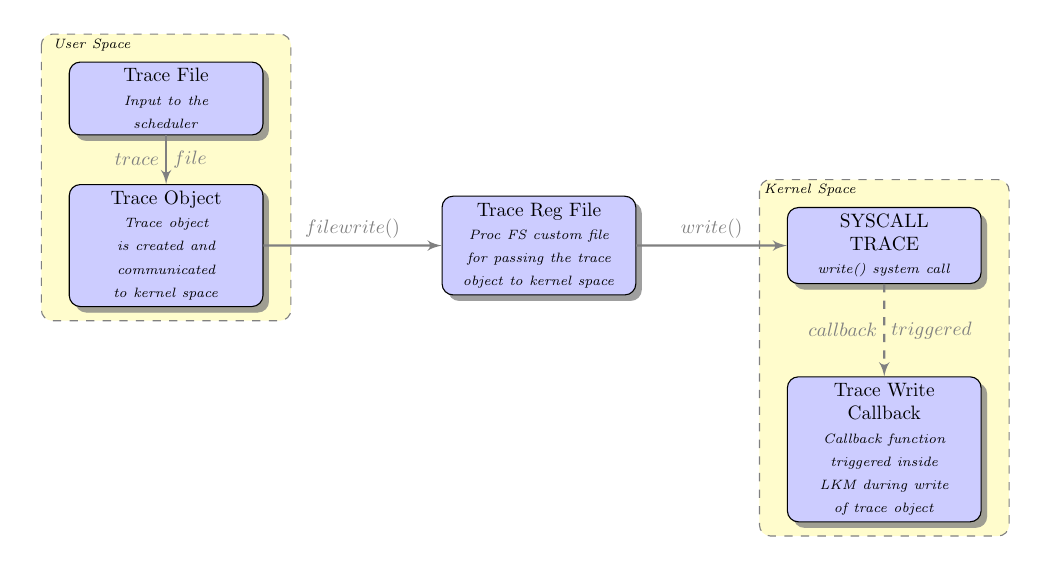
\begin{tikzpicture}[scale=0.7,transform shape]
 
  % Draw diagram elements
  % trace registration area
  \path \spacelayer {TRACEFILE}{Trace File}{Input to the scheduler};  
  \path (TRACEFILE.south)+(0.0,-2.0)\spacelayer {TRACEOBJ}{Trace Object}{Trace object is created and communicated to kernel space};  
  \path (TRACEOBJ.east)+(5.0,0.0) \spacelayer {TRACEPROCFS}{Trace Reg File}{Proc FS custom file for passing the trace object to kernel space};
  \path (TRACEPROCFS.east)+(4.5,0.0) \spacelayer {TRACESYSCALL}{SYSCALL\\ TRACE}{write() system call};  
  \path (TRACESYSCALL.south)+(0.0,-3.0) \spacelayer {TRACECALLBACK}{Trace Write Callback}{Callback function triggered inside LKM during write of trace object};
  
  % Draw arrows between elements

  %thread registration block
  \path [line] (TRACEFILE.south) -- node [left] {$trace$}
									 node [right] {$file$} (TRACEOBJ);
  \path [line] (TRACEOBJ.east) -- node [above] {$filewrite()$} (TRACEPROCFS);

  \path [line] (TRACEPROCFS.east) -- node [above] {$write()$} (TRACESYSCALL);
  
  \path [linepart] (TRACESYSCALL.south) -- node [left] {$callback$}
                                 node [right]{$triggered$} (TRACECALLBACK);  
  
  %background generation block
  \background{TRACEFILE}{TRACEFILE}{TRACEOBJ}{TRACEOBJ}{User Space}
  \background{TRACESYSCALL}{TRACESYSCALL}{TRACECALLBACK}{TRACECALLBACK}{Kernel Space}

\end{tikzpicture}

The trace file is passed on as an input for the scheduler. 
In the above flow diagram, the trace file is read by the main user thread at the start of its execution. 
It parses the file, creates and passes the trace object to the kernel space as string via a custom file created in the proc file system. 

\begin{algorithmic}
\If {$i\geq maxval$}
    \State $i\gets 0$
\Else
    \If {$i+k\leq maxval$}
        \State $i\gets i+k$
    \EndIf
\EndIf
\end{algorithmic}
\newpage
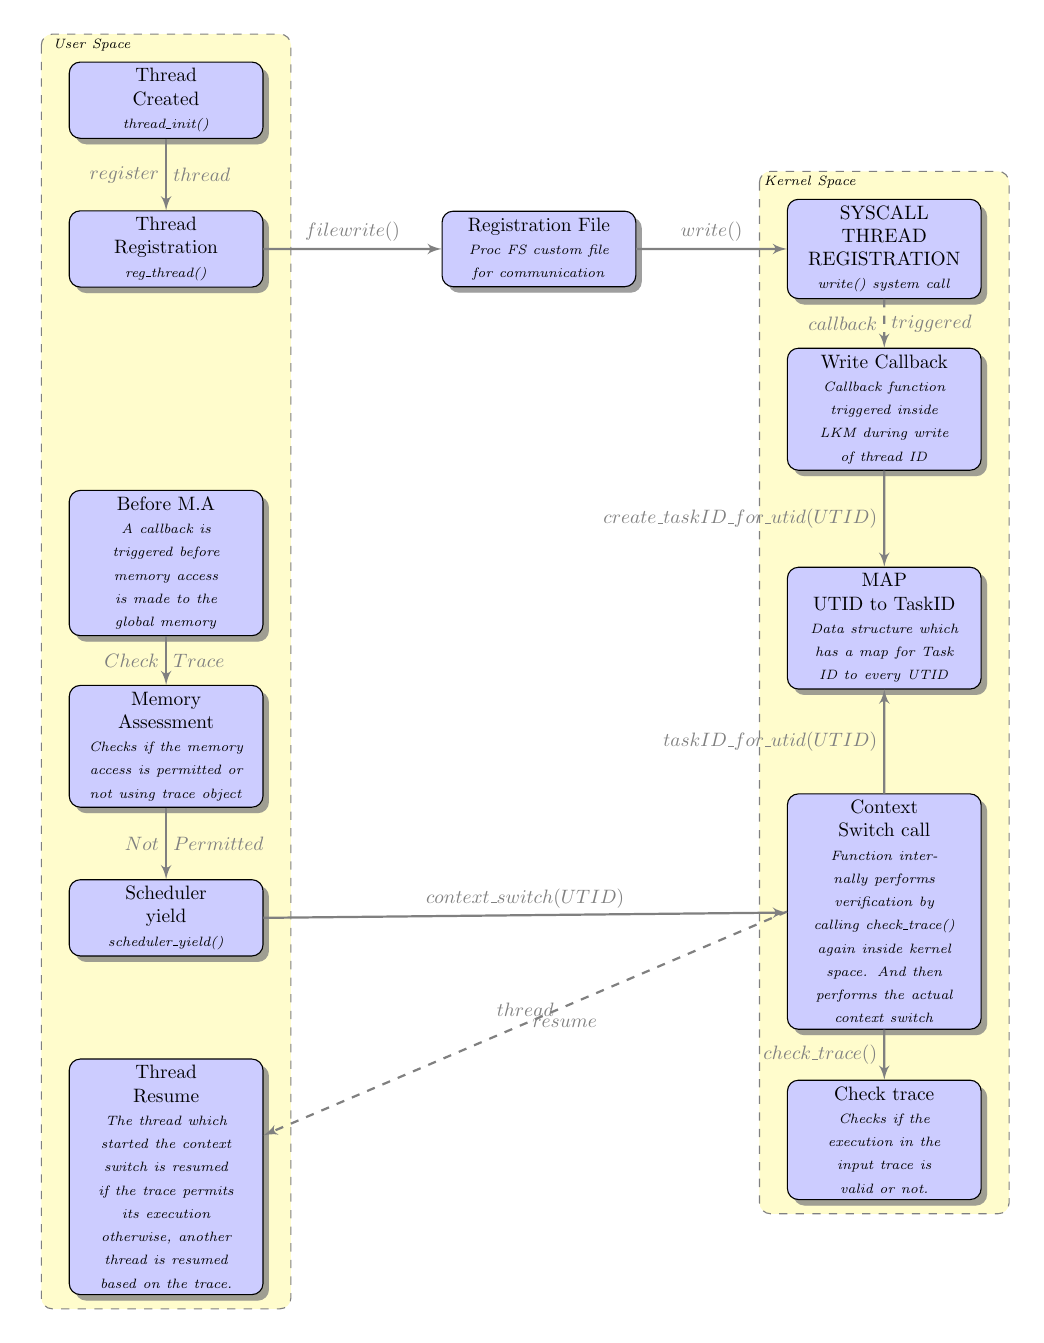
\begin{tikzpicture}[scale=0.7,transform shape]
 
 
  
  % thread registration block area
  \path \spacelayer {THREADINIT}{Thread\\ Created}{thread\_init()};  
  \path (THREADINIT.south)+(0.0,-2.0)\spacelayer {USERTHREADREG}{Thread\\ Registration}{reg\_thread()};  
  \path (USERTHREADREG.east)+(5.0,0.0) \spacelayer {REGPROCFS}{Registration File}{Proc FS custom file for communication};
  \path (REGPROCFS.east)+(4.5,0.0) \spacelayer {REGSYSCALL}{SYSCALL\\ THREAD\\ REGISTRATION}{write() system call};
  \path (REGSYSCALL.south)+(0.0,-2.0) \spacelayer {REGCALLBACK}{Write Callback}{Callback function triggered inside LKM during write of thread ID};

  % memory assessment area
  
  \path (USERTHREADREG.south)+(0.0,-5.0) \spacelayer {BEFOREMA}{Before M.A}{A callback is triggered before memory access is made to the global memory};
  \path (BEFOREMA.south)+(0.0,-2.0) \spacelayer {MEMASSESSMENT}{Memory\\ Assessment}{Checks if the memory access is permitted or not using trace object};
  \path (MEMASSESSMENT.south)+(0.0,-2.0) \spacelayer {SCHEDYIELD}{Scheduler\\ yield}{scheduler\_yield()};
  
  \path (SCHEDYIELD.south)+(0.0,-4.0) \spacelayer {THREADRESUME}{Thread\\ Resume}{The thread which started the context switch is resumed if the trace permits its execution otherwise, another thread is resumed based on the trace.};
  
  \path (REGCALLBACK.south)+(0.0,-8.0) \spacelayer {CONTEXTSWITCH}{Context Switch call}{Function internally performs verification by calling check\_trace() again inside kernel space. And then performs the actual context switch}; 
  \path (CONTEXTSWITCH.south)+(0.0,-2.0) \spacelayer {CHECKTRACE}{Check trace}{Checks if the execution in the input trace is valid or not.}; 
  \path (CONTEXTSWITCH.north)+(0.0,3.0) \spacelayer {MAPDATASTRUCTURE}{MAP\\ UTID to TaskID }{Data structure which has a map for Task ID to every UTID};
  
  

  % Draw arrows between elements

 
  %thread registration block
  \path [line] (THREADINIT.south) -- node [left] {$register$}
									 node [right] {$thread$} (USERTHREADREG);
  \path [line] (USERTHREADREG.east) -- node [above] {$filewrite()$} (REGPROCFS);

  \path [line] (REGPROCFS.east) -- node [above] {$write()$} (REGSYSCALL);
  
  \path [linepart] (REGSYSCALL.south) -- node [left] {$callback$}
                                 node [right]{$triggered$} (REGCALLBACK);
  \path [line] (REGCALLBACK.south) -- node [left] {$create\_taskID\_for\_utid(UTID)$} (MAPDATASTRUCTURE);                                 

  %memory assessment block
  \path [line] (BEFOREMA.south) -- node [left] {$Check$}
						     node [right] {$Trace$} (MEMASSESSMENT);

  \path [line] (MEMASSESSMENT.south) -- node [left] {$Not$}
						     node [right] {$Permitted$} (SCHEDYIELD);

  \path [line] (SCHEDYIELD.east) -- node [above] {$context\_switch(UTID)$} (CONTEXTSWITCH);
  
  \path [line] (CONTEXTSWITCH.south) -- node [left] {$check\_trace()$} (CHECKTRACE);
  
  \path [line] (CONTEXTSWITCH.north) -- node [left] {$taskID\_for\_utid(UTID)$} (MAPDATASTRUCTURE);

  \path [linepart] (CONTEXTSWITCH.west) -- node [above] {$thread$}
                                 node [right]{$resume$} (THREADRESUME);

  %background generation block
 
  \background{THREADINIT}{THREADINIT}{THREADRESUME}{THREADRESUME}{User Space}
  \background{REGSYSCALL}{REGSYSCALL}{CHECKTRACE}{CHECKTRACE}{Kernel Space}
  

\end{tikzpicture}

In the above picture, the registration block happens when a user thread is created. 
The registration happens via a custom proc file system. 
In the memory assessment block, the user thread initially performs a check of permissions to access memory. 
The check happens with the help of the trace object created from the trace input file. 
The memory assessment block is involved whenever there is a global memory event. 
Based on the assessment in kernel space, the assessment thread is resumed or another thread which was paused would be resumed. 

\end{document} 